\chapteruaf{The Plan}

\section{Motivation and Goals}

	With the increase in the use of VMI (drop your citations in here) in research settings as well as the migration of VMI to the commercial sphere ~\cite{_vmware_2014} the study of the security of this technique has taken on paramount importance. With the use of VMI to extract cryptographic keys from live memory ~\cite{hay_circumventing_2012} the dangers of misuse of VMI have become apparent. TODO (REWORD). 

	In this dissertation we have two goals

	\begin{enumerate}
	\item To detect the use of VMI on the guest VM from within the VM. 
	\item To , in some way, impair the use of VMI on the guest VM. 
	\end{enumerate} 

	For the detection of VMI we aim to determine if VMI is being run on the guest in any capacity. Our threshold for successful detection is a simple yes or no answer to the question ``Can the guest detect that it is being monitored by VMI?'' Any results which exceed this threshold will also be taken as confirmation of detection of VMI.

For the goal of impairing or subverting VMI we take as the threshold for success any  results which will affect the availability or integrity of the VMI agent being tested. 


\section{Threat Model}
	We begin defining the Trusted Computing Base (TCB) as the set of all hardware and software which is essential to the security of a computer system ~\cite{rushby_critical_1994}. Vulnerabilities in the TCB will be considered vunerabilities in the whole of the system. Components outside the TCB should not be able to elevate privileges than they are granted by the OS or hypervisor. 

	For the following experiments we will assume that the hypervisor as well as all associated interfaces such as libvirt or xencntrl are part of the TCB. All VMI agents will also be assumed to be part of the TCB. The guest VM will be outside of the TCB and therefore all malicious code must be executed on the guest VM. We further assume that the malicious VM is isolated from all other VMs. 

	The attacker on the malicious VM will be assumed to have root access to the VM and therefore will be allowed to install malicious kernel modules as well as run malicious user code. 

\section{Experimental Setup}\label{Apparatus}

	The hosts in our experiments will use version 4.2 of Xen~\cite{barham_xen_2003} and version 3.2.0 of KVM ~\cite{kivity_kvm:_2007}along with version 1.6.2 of QEMU~\cite{bellard_qemu_2005} (the userspace component to KVM). Guests are Ubuntu Server VMs with Linux kernel version 3.11.0-12-generic~\cite{_Linux_archive}. Guests are allocated 1GB of RAM and 1VCPU. Unless otherwise stated all VMs are clones of the original VM created. 

	For experiments concerning the detection of VMI a simple system will be used where one guest VM is run on a physical host system ~\ref{ExpApp}. 

	\begin{figure}\label{ExpApp}
	  \centering
	  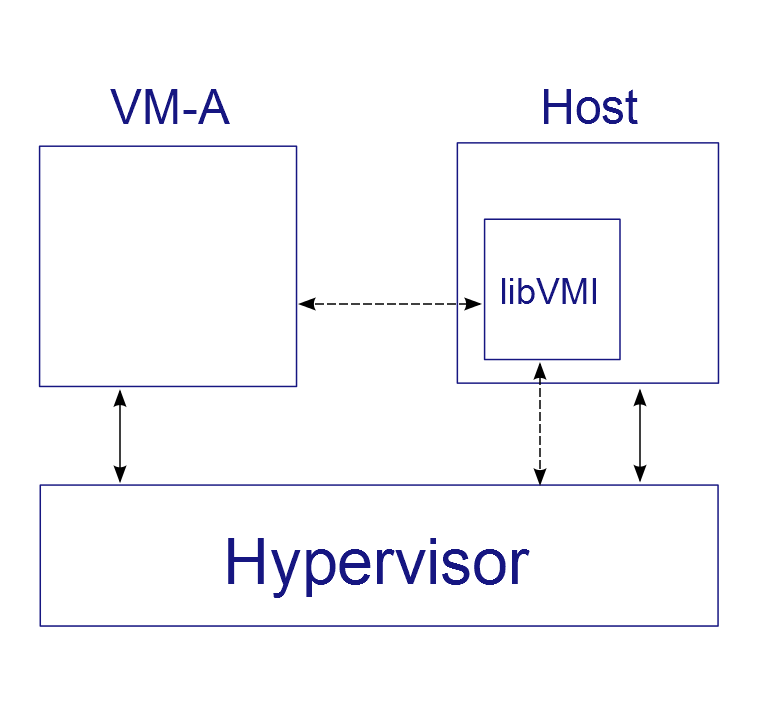
\includegraphics[width=\textwidth]{figures/BM_graph3_cropped.png}
	  \caption{Experimental Setup}
	\end{figure}

\section{VMI Agents}
For the detection of VMI all experiments will be using VMITools~\cite{payne_vmitools_2014}. Since the primary means of doing VMI is to copy a page from memory then interpret it [cite a few], any toolsuite which does this can be used for this experiment without the loss of generality. There will be three VMI programs used for these experiments; map-addr, process-list, and module-list. 

The map-addr program simply maps an address from the guests memory to the memory of the VMI agent. The process-list command maps the processes currently running on a VM. In Linux the list of running processes is stored in the task-list (cite sched.h). The task list is a doubly linked list where each node in the list represents a process being handled by the OS. The process-list program begins by mapping the head node of the task list from the guest to the VMI agent. The first task struct is then decoded. The desired information , such as pids and process names, is displayed to the user and the location of the next task in the list is recorded. The next node in the task list is processed in the same way. This continues until the list comes back to the head of the task list, indicating that the entire list has been traversed. 


\begin{algorithm}[p]\label{ProcList}
	\SetAlgoLined
	\KwResult{A list of the processes running on a target VM}
	current\_task = Domain.task\_list\_head\;
	\Repeat{current\_task.adr==Domain.task\_list\_head.adr}	
	{
	 	adr=current\_task.nextTask.adr \;
	 	map Task Struct at adr to host \;
	 	translate nextTaskStruct 	   \;
	 	current\_task = taskStruct at adr \;
	}
	\caption{The Process-List Program}
\end{algorithm}


\begin{algorithm}[p]\label{ModList}
	\SetAlgoLined
	\KwResult{A list of the Module running on a target VM}
	current\_module = Domain.module\_list\_head\;
	\Repeat{current\_module.adr==Domain.module\_list\_head.adr}	
	{
	 	adr=current\_task.nextModule.adr \;
	 	map Module Struct at adr to host \;
	 	translate nextModuleStruct 	   \;
	 	current\_Module = ModuleStruct at adr \;
	}
	\caption{The Module-List Program}
\end{algorithm}



The module list works in much the same way. 


\section{Experiments}
In this dissertation we propose five experiments. Four experiments will be used to detect VMI and the last will be an attempt to subvert VMI by gaining control of the host through the VMI channel. 

For our first experiment we wish to analyze data produced by the Linux utility Sysstat~\cite{godard_sysstat_2010}. Sysstat measures over 200 (TODO Figure out the right amount) fields used by Linux such as page faults per second, context switches per second, and percentage of swap space used. Since the host, guest, and VMI agent all use the same physical resources it is possible that the patterns can emerge in those numbers which can identify the use of VMI on the guest. 

For our second experiment we propose to analyze the time it takes to map and unmap a page in memory. With main memory and the page table being shared between VMs,  it's possible that the use of a VMI agent on the guest will cause a distinguishable difference in the time taken to do the mapping and unmapping of a page.

Our third experiment is similar to the first experiment in that in memory timing is used to determine if a guest is being monitored by VMI. In this case it's the use of the CPU cache. If they are on the same CPU a guest and a VMI agent will share the same L3 cache. If they are on the same core they will share the same L2 and L1 cache as well. For our experiment we propose measuring how long it takes to write an element in memory. Between each measurement we flush all three caches. We hypothesize there will be a small dip in the time required to access memory after it has been flushed from cache if a VMI agent has been accessing memory in that program. (TODO FIX to make specific about the page being monitored) 


Our fourth experiment takes advantage of the fact that KVM uses several features of the Linux kernel. In this case the scheduler and the KSM mechanism. KVM uses the Linux scheduler, in this case the Completely Fair Scheduler (CFS) ~\cite{pabla_completely_2009}, to manage VMs essentially as Linux processes. As a result of being treated as Linux processes, KVM VMs are subject to memory de-duplication using KSM. We hypothesize that the memory de-duplication can be measured as in ~\cite{xiao_security_2013}~\cite{owens_non-interactive_2011} if a VMI agent copies a page from the guest's memory to the host's memory.

\section{On Timing}

In this chapter we will be discussing the analysis of a number of different timings. For these timings we used the C++11 chrono object~\cite{_chrono_2014}. The C++ chrono object offers a high-resolution timer, the resolution of which is dependent on the system. In Linux the high-resolution timer offers nanosecond resolution.  In order to determine the resolution and any computational overhead for the chrono object we take a sample inside the guest VM. In this sample we simply run take two time measurements one after the other and log the difference between them. We take 1,000,000 measurements like this and plot them Figure ~\ref{RawTiming}. What we see is that while we have nanosecond resolution there is a significant amount of overhead involved in the start of a timing measurement. In order to compensate for this we take the minimum value of our measurements and subtract it from all subsequent measurements. 

\begin{figure}\label{RawTiming}
	  \centering
	  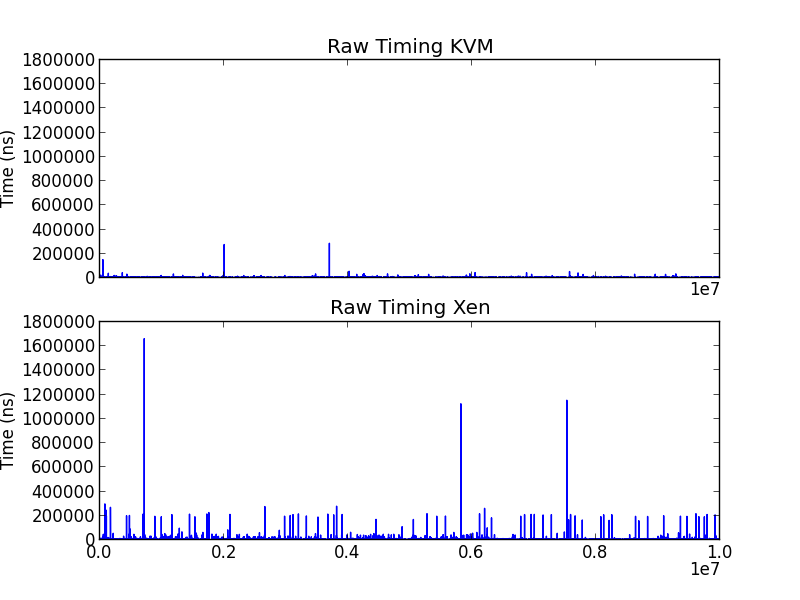
\includegraphics[width=\textwidth]{figures/RawTimingXenandKVM.png}
	  \caption{Raw Timing for Xen and KVM}
\end{figure}


The minimum value is quite close in both KVM and Xen at 549 ns and 539 ns respectively. These measurements represent the bare minimum amount of time it takes to perform a timing measurement so we can subtract it as overhead on subsequent measurements.  